\section{Access Control Hardware/Software Implementation}
\begin{figure}[H]
  \centering
  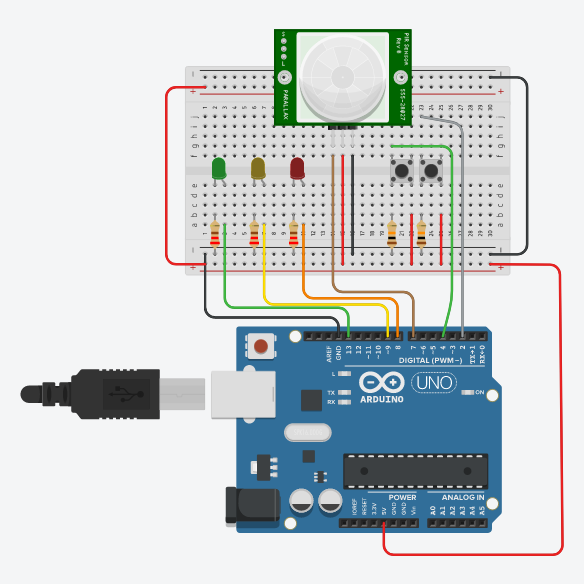
\includegraphics[scale=0.5]{figs/ArduinoSnapshot.png}
  \caption{Arduino wiring diagram}
  \label{fig:Arduino}
\end{figure}

\textbf{Hardware:}

The system has 3 signaling LEDs for showing the current system state. It also has two impulse push buttons used to input the access code. Finally it has a PIR detector that senses movement and signals this to the Arduino board. Everything is connected to the digital I/O.\\

The LEDs and input buttons all have current limiting resistors connected in series with them to prevent damaging them. This actually isn't necessary in the software simulation as they are indestructible. \\
\\
\textbf{Software:}

The Arduino runs through the setup() function before running the loop() function until the device is turned off. The speed of the system makes the loop function complete several thousand times per second, because of this we need to save if we detected button presses and inputs as these can be pressed for several loops without an intended new input.\\
 
In the setup we set all the pin-modes for all the inputs and outputs we are using. For this task we only needed to use the digital inputs and outputs. These all receive/output either a HIGH or LOW signal. After the setup call, we create a few constants and variables to store information outside of the loop.\\

In the loop we first retrieve the states of the inputs. After that we check if the PIR detector input is HIGH and if we previously managed this event. If this is a new input we change the system to the waiting state, and save that we managed the input. 

After this we enter a switch statement which performs different tasks depending on the set system state. In all the states, we refresh the outputs so they are correct for the systems current state. This is necessary because the system might have changed state. \\

In the waiting state we check if any of the buttons have been pressed, and if the last pressed button is a valid one. Doing this we can implement a simple code checking. We also pulse the Yellow LED so the user can see the input has been detected. The pulsing has to be done with a delay() call between the output states, as it would not be noticeable that the LED blinked by humans without it.\\

The code doesn't implement any actuator locking or unlocking, but this would simply be a line of code contained in each of the  switch cases. 
\pagebreak